\documentclass[10pt,a4paper]{article}
\usepackage[margin=0.6in,top=0.5in,bottom=0.5in]{geometry}
\usepackage{amsmath,amssymb,amsfonts}
\usepackage{braket}
\usepackage{graphicx}
\usepackage{xcolor}
\usepackage{enumitem}
\usepackage{tcolorbox}
\usepackage{multicol}
\usepackage{hyperref}
\usepackage{fancyhdr}
\usepackage{tikz}
\usepackage{booktabs}
\usepackage{caption}
\usepackage{float}
\usepackage{tabularx}

% Color definitions
\definecolor{deepblue}{RGB}{0,51,102}
\definecolor{alertred}{RGB}{180,30,30}
\definecolor{progreen}{RGB}{0,100,50}
\definecolor{conred}{RGB}{160,40,40}
\definecolor{keyorange}{RGB}{200,100,0}
\definecolor{mathpurple}{RGB}{100,0,130}
\definecolor{lightblue}{RGB}{220,235,255}
\definecolor{lightyellow}{RGB}{255,255,220}
\definecolor{lightgreen}{RGB}{220,255,220}
\definecolor{lightred}{RGB}{255,225,225}
\definecolor{boxgray}{RGB}{240,240,240}

% tcolorbox styles
\tcbuselibrary{skins,breakable}

\newtcolorbox{algorithmbox}[1]{
  colback=lightblue,
  colframe=deepblue,
  fonttitle=\bfseries\color{deepblue},
  title={#1},
  breakable,
  sharp corners,
  boxrule=1.2pt,
  left=4pt,right=4pt,top=2pt,bottom=2pt
}

\newtcolorbox{prosbox}{
  colback=lightgreen,
  colframe=progreen,
  fonttitle=\bfseries\color{progreen},
  title={\textcolor{progreen}{\textbf{$\boldsymbol{+}$ Pros}}},
  sharp corners,
  boxrule=0.8pt,
  left=3pt,right=3pt,top=2pt,bottom=2pt
}

\newtcolorbox{consbox}{
  colback=lightred,
  colframe=conred,
  fonttitle=\bfseries\color{conred},
  title={\textcolor{conred}{\textbf{$\boldsymbol{-}$ Cons}}},
  sharp corners,
  boxrule=0.8pt,
  left=3pt,right=3pt,top=2pt,bottom=2pt
}

\newtcolorbox{insightbox}{
  colback=lightyellow,
  colframe=keyorange,
  fonttitle=\bfseries\color{keyorange},
  title={\textcolor{keyorange}{\textbf{Expert Intuition}}},
  breakable,
  sharp corners,
  boxrule=0.8pt,
  left=3pt,right=3pt,top=2pt,bottom=2pt
}

\newtcolorbox{keybox}{
  colback=boxgray,
  colframe=black!50,
  sharp corners,
  boxrule=0.5pt,
  left=3pt,right=3pt,top=2pt,bottom=2pt
}

% Compact lists
\setlist[itemize]{noitemsep,topsep=1pt,leftmargin=12pt}
\setlist[enumerate]{noitemsep,topsep=1pt,leftmargin=14pt}

% Smaller section fonts
\usepackage{titlesec}
\titleformat{\section}{\large\bfseries\color{deepblue}}{\thesection}{0.5em}{}
\titleformat{\subsection}{\normalsize\bfseries\color{deepblue!80}}{\thesubsection}{0.5em}{}
\titleformat{\subsubsection}{\small\bfseries\color{deepblue!60}}{\thesubsubsection}{0.5em}{}
\titlespacing*{\section}{0pt}{6pt}{3pt}
\titlespacing*{\subsection}{0pt}{4pt}{2pt}
\titlespacing*{\subsubsection}{0pt}{3pt}{1pt}

\setlength{\parindent}{0pt}
\setlength{\parskip}{2pt}

\graphicspath{{figures/tripathi/}}

\pagestyle{fancy}
\fancyhf{}
\fancyhead[L]{\small\textcolor{deepblue}{Tripathi et al. --- Benchmarking Quantum Gates \& Circuits}}
\fancyhead[R]{\small\thepage}
\renewcommand{\headrulewidth}{0.4pt}

\begin{document}

% ===========================================================================
% TITLE PAGE / INDEX
% ===========================================================================
\begin{center}
{\LARGE\bfseries\textcolor{deepblue}{Benchmarking Quantum Gates and Circuits}}\\[4pt]
{\normalsize Tripathi, Kowsari, Saurav, Zhang, Levenson-Falk \& Lidar (2025)}\\[2pt]
{\small arXiv:2407.09942v2 $\mid$ USC, Center for Quantum Information Science \& Technology}\\[6pt]
{\small\textcolor{gray}{Comprehensive Summary with Expert Intuition}}
\end{center}
\vspace{4pt}
\hrule height 1pt
\vspace{8pt}

\tableofcontents
\vspace{6pt}
\hrule height 0.5pt

% Legend
\vspace{4pt}
\begin{center}
\small
\colorbox{lightblue}{\textcolor{deepblue}{\textbf{Algorithm/Protocol}}} \quad
\colorbox{lightgreen}{\textcolor{progreen}{\textbf{Pros}}} \quad
\colorbox{lightred}{\textcolor{conred}{\textbf{Cons}}} \quad
\colorbox{lightyellow}{\textcolor{keyorange}{\textbf{Expert Intuition}}} \quad
\textcolor{alertred}{\textbf{Key result}} \quad
\textcolor{mathpurple}{\textbf{Math detail}}
\end{center}

\newpage

% ===========================================================================
% SECTION 1: INTRODUCTION
% ===========================================================================
\section{Introduction and Motivation}

\begin{itemize}
  \item Fault-tolerant quantum computing requires \textcolor{alertred}{gate fidelities exceeding accuracy thresholds} ($p_{\text{err}} < 10^{-4}$ for chemical accuracy, $10^{-5}\text{--}10^{-6}$ for dynamics)
  \item \textbf{Gate errors} are a fundamental bottleneck --- each extra order of magnitude in fidelity $\Rightarrow$ disproportionately lower qubit counts / circuit depths
  \item This paper: review of \textcolor{deepblue}{6 major benchmarking methods} + introduction of \textcolor{alertred}{Deterministic Benchmarking (DB)}, a novel protocol
  \item Part of the broader field of \textbf{QCVV} (Quantum Characterization, Verification \& Validation)
\end{itemize}

\begin{insightbox}
\begin{itemize}
  \item \textbf{Why benchmarking matters for chemistry}: VQE/QPE require gate decompositions that preserve coherence over large circuit depths; any fidelity deviation biases energy predictions
  \item \textbf{Coherent vs.\ incoherent}: Coherent errors add as \emph{amplitudes} (quadratically worse), incoherent add as \emph{probabilities}. Traditional RB deliberately randomizes noise $\Rightarrow$ can miss coherent errors
  \item \textbf{Philosophy}: No single benchmarking method is universally best --- the trade-off is always \emph{comprehensiveness vs.\ resource cost vs.\ simplicity}
  \item Not covered in this review: cycle benchmarking, quantum volume, mirror benchmarking, ML-based benchmarking, EPLG, etc.\ (these are mostly variants of the core methods reviewed here)
\end{itemize}
\end{insightbox}

\newpage

% ===========================================================================
% SECTION 2: GATE ERRORS
% ===========================================================================
\section{Gate Errors}

\subsection{Quantum Dynamical Maps}

\begin{itemize}
  \item A quantum process (channel) $\mathcal{E}$ is a \textbf{CPTP map}: $\mathcal{E}(\rho) = \sum_i A_i \rho A_i^\dagger$, with $\sum_i A_i^\dagger A_i = I$
  \item \textcolor{mathpurple}{\textbf{Process matrix $\chi$}}: Expand Kraus operators in a fixed Hermitian basis $\{E_m\}_{m=0}^{D^2-1}$ satisfying $\mathrm{Tr}(E_m^\dagger E_n) = D\,\delta_{mn}$:
  \begin{equation}
    \mathcal{E}(\rho) = \sum_{m,n=0}^{D^2-1} \chi_{mn}\, E_m\, \rho\, E_n^\dagger, \qquad \chi_{mn} = \sum_i a_{in}^* a_{im} = \chi_{nm}^*
  \end{equation}
  $\chi$ is Hermitian, positive semidefinite; encodes \textcolor{alertred}{$D^4 - D^2$ real parameters} (12 for a single qubit)
  \item \textbf{Choi--Jamio\l{}kowski isomorphism}: Map $\mathcal{E} \leftrightarrow$ Choi state $\rho_\mathcal{E} = (I \otimes \mathcal{E})(|\phi\rangle\langle\phi|)$ where $|\phi\rangle = \frac{1}{\sqrt{D}}\sum_i |i\rangle \otimes |i\rangle$
  \item \textcolor{mathpurple}{\textbf{Process fidelity}}: $F_{\mathrm{proc}}(\mathcal{E}, \mathcal{E}') = F(\rho_\mathcal{E}, \rho_{\mathcal{E}'}) = \|\sqrt{\rho_\mathcal{E}}\sqrt{\rho_{\mathcal{E}'}}\|_1$ (Uhlmann fidelity between Choi states)
\end{itemize}

\subsection{Coherent vs.\ Incoherent Errors}\label{sec:coherent-incoherent}

\begin{keybox}
\begin{tabular}{p{0.46\textwidth}|p{0.46\textwidth}}
\textcolor{alertred}{\textbf{Coherent Errors}} & \textcolor{deepblue}{\textbf{Incoherent Errors}} \\
\midrule
Purity preserved: $\mathrm{Tr}(\rho^2) = 1$ & Purity lost: $\mathrm{Tr}(\rho^2) < 1$ \\
Deterministic, repeatable & Random (stochastic) \\
Amplitudes add in phase $\Rightarrow$ failure prob.\ grows \textcolor{alertred}{quadratically} & Probabilities add $\Rightarrow$ failure prob.\ grows linearly \\
Always reversible in principle & Requires QEC to reverse \\
More damaging in general & \\
\end{tabular}
\end{keybox}

\subsection{Single-Qubit Gate Errors}

Bloch vector $\vec{v} = (\langle\sigma_x\rangle, \langle\sigma_y\rangle, \langle\sigma_z\rangle)$; general gate $R(\vartheta, \theta, \phi)$ = rotation by $\vartheta$ about axis $(\theta,\phi)$.

\textcolor{alertred}{\textbf{Coherent errors:}}
\begin{itemize}
  \item \textbf{Rotation errors}: $\vartheta$ deviates from target (drive amplitude drifts, coupling errors)
  \item \textbf{Phase errors}: rotation axis altered ($\theta$ and/or $\phi$ change); from qubit frequency drifts, control phase drifts
  \item \textbf{Leakage}: state evolves outside qubit space (e.g., transmon higher levels); coherent if it preserves purity
\end{itemize}

\textcolor{deepblue}{\textbf{Incoherent errors:}}
\begin{itemize}
  \item \textbf{Relaxation ($T_1$)}: bit-flip errors, exponential decay toward equilibrium; nonzero purity at finite $T$
  \item \textbf{Dephasing ($T_2$, $T_\phi$)}: phase-flip errors; Markovian + $1/f$ noise components common in solid-state; $1/T_2 = 1/(2T_1) + 1/T_\phi$
  \item \textbf{Erasure}: special leakage where qubit info lost with a known signature; easier to correct than general errors
\end{itemize}

\textcolor{mathpurple}{\textbf{Depolarizing model}} (lumps incoherent errors):
\begin{equation}
  \mathcal{E}(\rho) = (1-p)\rho + \frac{p}{3}(X\rho X + Y\rho Y + Z\rho Z)
\end{equation}
\textcolor{alertred}{Limitation}: obscures physical origin, ignores biased noise \& finite temperature.

\textbf{Total parameter count} (Markovian, ignoring erasure): \textcolor{alertred}{7 parameters} --- $\delta\vartheta$, $\delta\theta$, $\delta\phi$, $\gamma_1$ (relaxation), equilibrium population, $\gamma_\phi$ (dephasing), leakage angle.

\subsection{Two-Qubit Gate Errors}

\begin{itemize}
  \item Error landscape is \emph{much richer} than single-qubit: device/implementation specific
  \item Example (parametrically-activated iSWAP in transmons): errors include $T_1$/$T_2$ of each qubit, $1/f$ dephasing, coupler noise, incomplete swapping, $ZZ$ interaction, phase errors, leakage
  \item \textbf{Best practice}: develop an ``error budget''; full QPT once, then targeted measurements
  \item \textbf{Key danger}: amplification of single-qubit coherent errors when amplifying two-qubit errors --- use dynamical decoupling between gate applications
  \item Two-qubit incoherent errors (joint bath couplings) are often ignored but can be significant (e.g., coupler as joint bath)
\end{itemize}

\newpage

% ===========================================================================
% SECTION 3: BENCHMARKING PROTOCOLS
% ===========================================================================
\section{Gate and Circuit Benchmarking Protocols}

\textbf{Criteria for judging a benchmarking protocol:}
\begin{enumerate}
  \item \textcolor{deepblue}{\textbf{Comprehensiveness}}: How much error information? (number of parameters characterized)
  \item \textcolor{deepblue}{\textbf{Specificity}}: What noise model assumptions? (gate-independent? Pauli? etc.)
  \item \textcolor{deepblue}{\textbf{Simplicity}}: How easily adapted to existing setups?
  \item \textcolor{deepblue}{\textbf{Resource cost}}: How expensive to run? (number of circuits, measurements, classical post-processing)
  \item \textcolor{deepblue}{\textbf{Robustness to SPAM}}: Critical requirement for most protocols
\end{enumerate}

\newpage

% ---------------------------------------------------------------------------
% 3.1 RANDOMIZED BENCHMARKING
% ---------------------------------------------------------------------------
\subsection{Randomized Benchmarking (RB)}

\subsubsection{Standard RB}

\begin{algorithmbox}{Standard RB Protocol}
\begin{enumerate}
  \item \textbf{Prepare} $|0\rangle^{\otimes n}$
  \item \textbf{Apply} $m$ random Clifford gates $\{C_i\}_{i=1}^m$: \quad $U_m = C_m C_{m-1}\cdots C_1$
  \item \textbf{Inversion gate}: $C_{\mathrm{inv}} = C_{m+1} = U_m^\dagger = C_1^\dagger \cdots C_m^\dagger$ \quad (efficiently computable classically)
  \item \textbf{Measure} in computational basis; record if system returned to $|0\rangle^{\otimes n}$
  \item \textbf{Average} over $K$ random sequences at each depth $m$ $\Rightarrow$ survival probability $P(m)$
  \item \textbf{Fit}: $P_{\mathrm{avg}}(m) = A\,p^m + B$ \quad to extract depolarization parameter $p$
\end{enumerate}
\end{algorithmbox}

\textbf{Groups}: \textbf{Pauli group} $\mathcal{P}_n$ = all $n$-fold tensor products of $\{I, X, Y, Z\}$. \textbf{Clifford group} = gates $C$ such that $C P C^\dagger \in \mathcal{P}_n$ for all $P \in \mathcal{P}_n$ (preserves Pauli group under conjugation).

\textcolor{alertred}{\textbf{Key idea:}} Random Clifford gates \emph{twirl} the error map into an effective \textbf{depolarizing channel}:
\begin{equation}
  \mathcal{E}_{\mathrm{dep}}(\rho) = p\,\rho + (1-p)\frac{I}{D}
\end{equation}

\textcolor{mathpurple}{\textbf{RB Theory:}} Assuming gate-independent noise $\mathcal{E}_i \equiv \mathcal{E}$:
\begin{equation}
P_{\mathrm{avg}}(m) = \mathrm{Tr}\!\left[\rho_0\, \mathcal{E}\!\left(p^m \rho_0 + (1-p^m)\frac{I}{D}\right)\right] = A\,p^m + B
\end{equation}
where $A = \mathrm{Tr}\!\left[\rho_0\,\mathcal{E}\!\left(\rho_0 - \frac{I}{D}\right)\right]$, $B = \mathrm{Tr}\!\left[\rho_0\,\mathcal{E}\!\left(\frac{I}{D}\right)\right]$.

$A$ and $B$ capture SPAM errors. \textcolor{alertred}{Average Clifford gate infidelity}:
\begin{equation}
  \boxed{r_C = \frac{D-1}{D}(1-p)}
\end{equation}

\textbf{Gate-dependent noise correction} (1st order):
$P_{\mathrm{avg}}^{(1)}(m) = A_1 p^m + B_1 + C_1(m-1)(q - p^2)p^{m-2}$; $(q-p^2)$ measures gate-dependence.

\subsubsection{Interleaved RB (IRB)}

\begin{algorithmbox}{Interleaved RB Protocol}
\begin{enumerate}
  \item Run \textbf{standard RB} $\Rightarrow$ extract decay parameter $p$
  \item Run \textbf{interleaved sequence}: insert target gate $G$ between every pair of random Cliffords:
  \[
    U_{m,\mathrm{inter}} = G_m \circ G \circ G_{m-1} \circ \cdots \circ G \circ G_2 \circ G \circ G_1
  \]
  followed by $G_{m+1} = U_{m,\mathrm{inter}}^{-1}$ $\Rightarrow$ extract $p_{\mathrm{inter}}$
  \item \textcolor{alertred}{Gate infidelity of $G$}: $r_G = \frac{D-1}{D}\left(1 - \frac{p_{\mathrm{inter}}}{p}\right)$
\end{enumerate}
\end{algorithmbox}

\textcolor{alertred}{\textbf{Caveat}}: Coherent errors in $G$ can \emph{add or cancel} with random Clifford errors $\Rightarrow$ possibly \textbf{negative} $r_G$ (unphysical $F > 1$). Error bound: $r_G \in [r_G - E, \, r_G + E]$ with
\[
E = \min\!\left\{\frac{(D-1)|p - p_{\mathrm{inter}}/p| + (1-p)}{D},\;\; \frac{2(D^2-1)(1-p)}{pD^2} + \frac{4\sqrt{1-p}\;\sqrt{D^2-1}}{pD^2}\right\}
\]

\textbf{Extensions of RB}: Simultaneous RB, Leakage RB, Non-Markovian RB, Mirror RB, Character RB (beyond Clifford group).

\begin{minipage}[t]{0.48\textwidth}
\begin{prosbox}
\begin{itemize}
  \item SPAM-robust (captured by $A$, $B$)
  \item Simple to implement; scalable
  \item Single-number summary useful for quick comparison
  \item Widely adopted, well understood theory
\end{itemize}
\end{prosbox}
\end{minipage}
\hfill
\begin{minipage}[t]{0.48\textwidth}
\begin{consbox}
\begin{itemize}
  \item Reduces error to a \emph{single number} --- loses all specificity
  \item Insensitive to coherent errors (twirling converts them to depolarizing)
  \item Assumes gate-independent, time-independent noise
  \item Gate-dependent corrections require large $m$ conflicting with validity conditions
\end{itemize}
\end{consbox}
\end{minipage}

\begin{insightbox}
\begin{itemize}
  \item RB is the ``quick health check'' of quantum gates --- tells you the \emph{average} error rate, but not \emph{what} is wrong
  \item The twirling trick is powerful but also RB's main weakness: by converting all noise to depolarizing, \textcolor{alertred}{coherent errors that may accumulate quadratically in circuits are rendered invisible}
  \item In practice, RB fidelity can look great while the actual circuit performance is poor because coherent error dominates
  \item IRB is unreliable when $p_{\mathrm{inter}} > p$; always check the error bound $E$
\end{itemize}
\end{insightbox}

\newpage

% ---------------------------------------------------------------------------
% 3.2 QUANTUM PROCESS TOMOGRAPHY
% ---------------------------------------------------------------------------
\subsection{Quantum Process Tomography (QPT)}

\subsubsection{Standard QPT (SQPT)}

\begin{algorithmbox}{Standard QPT Protocol}
\begin{enumerate}
  \item Prepare $D^2$ linearly independent input states $\{\rho_k\}$
  \item Apply the map $\mathcal{E}$ to each
  \item Perform quantum state tomography on each output $\mathcal{E}(\rho_k)$: measure expectations of $D^2$ basis operators $\{E_k\}$
  \item \textbf{Total measurements}: $D^4$
  \item Reconstruct $\chi$ via matrix inversion: $B\chi = \lambda$, where $B$ is $D^4 \times D^4$, $\lambda$ contains tomographic data
\end{enumerate}
\end{algorithmbox}

\textcolor{mathpurple}{\textbf{Key equations:}} Express $\mathcal{E}(\rho_k) = \sum_l \lambda_{kl}\,\rho_l$ with $\lambda_{kl} = \mathrm{Tr}(\rho_k\,\mathcal{E}(\rho_l))$. Expand $E_m \rho_k E_n^\dagger = \sum_l B_{mn,lk}\,\rho_l$. Then $\sum_{mn} B_{mn,lk}\,\chi_{mn} = \lambda_{kl}$.

\begin{figure}[H]
\centering
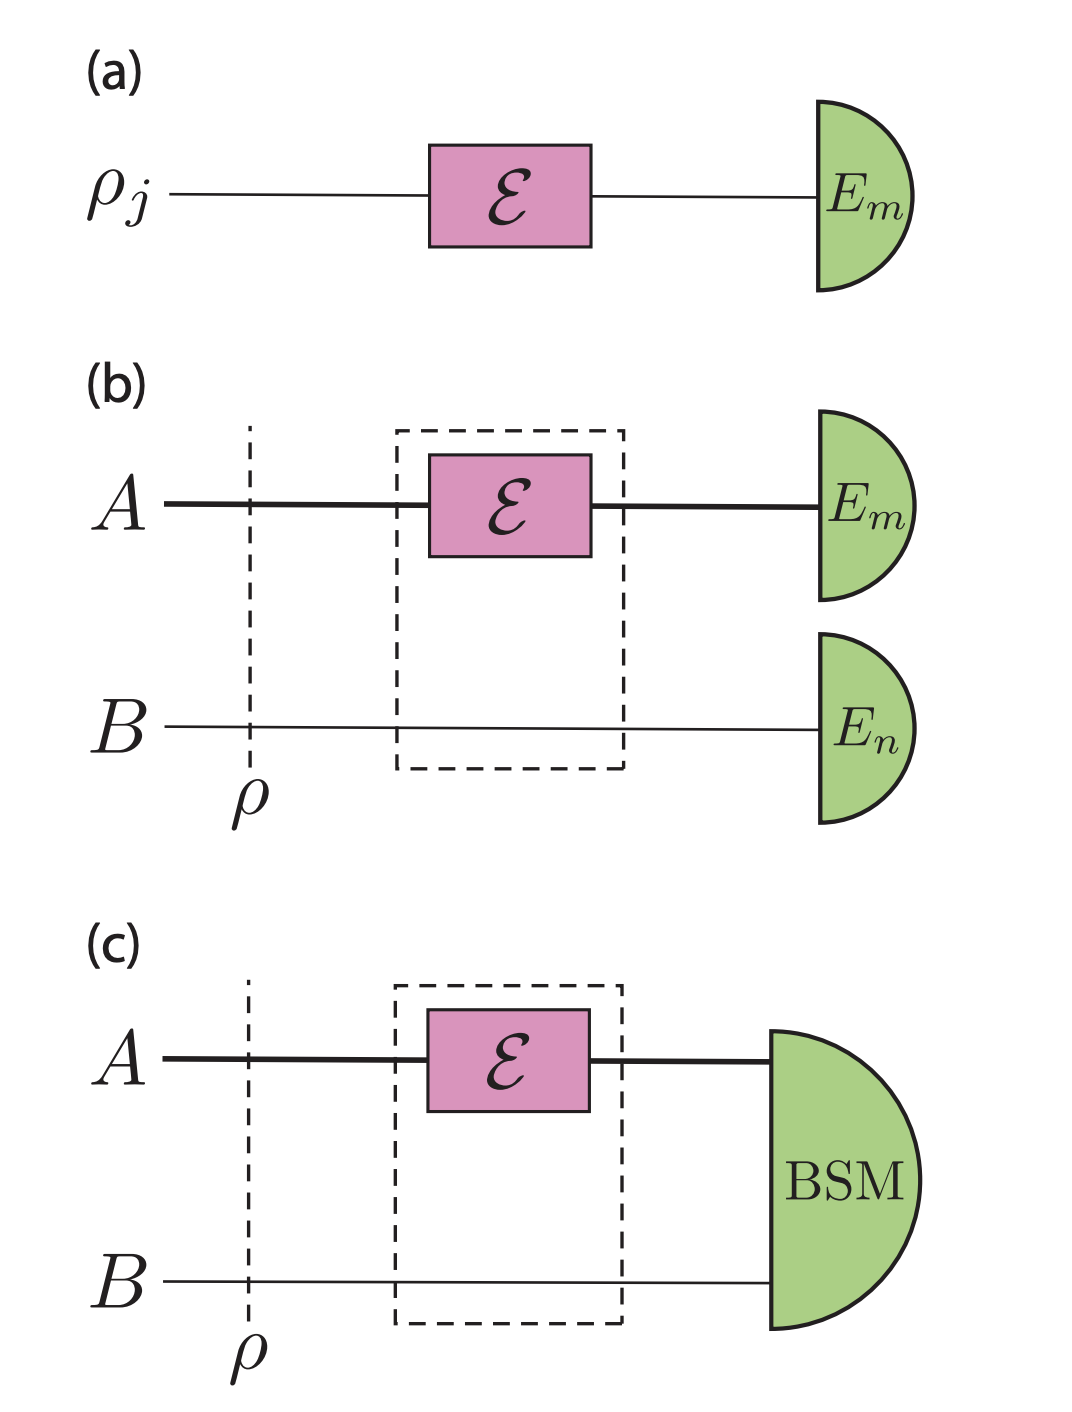
\includegraphics[width=0.45\textwidth]{fig1.png}
\caption{Three QPT variants: (a) SQPT, (b) Separable AAPT, (c) DCQD. Note DCQD uses Bell-state measurement.}
\end{figure}

\subsubsection{Ancilla-Assisted Process Tomography (AAPT)}

\begin{itemize}
  \item Based on \textbf{Choi--Jamio\l{}kowski isomorphism}: QPT $\equiv$ state tomography of the Choi state
  \item Attach ancilla $B$; prepare ``faithful'' joint state $\rho_{AB}$ (must have maximal Schmidt number $D^2$)
  \item Apply $\mathcal{E} \otimes I$ on the joint system; perform state tomography on output
  \item Reconstruct $\chi$ via \textbf{two matrix inversions}: $\tilde{\alpha} = \tilde{\chi}\,\varrho$ then invert to find $\chi$
  \item Maximally entangled states are \emph{optimal} (minimize experimental error amplification from matrix inversion)
  \item Separable vs.\ non-separable measurements: non-separable offers no practical advantage (requires many-body interactions)
\end{itemize}

\subsubsection{Direct Characterization of Quantum Dynamics (DCQD)}

\begin{algorithmbox}{DCQD Protocol (single qubit)}
\begin{enumerate}
  \item \textbf{Diagonal elements $\chi_{mm}$}: Prepare maximally entangled $|\Phi^+\rangle = \frac{1}{\sqrt{2}}(|00\rangle + |11\rangle)$; apply $\mathcal{E} \otimes I$; perform Bell-state measurement (BSM):
  \[
    \textcolor{alertred}{p_m = \mathrm{Tr}[P_m\, (\mathcal{E}\otimes I)(|\Phi^+\rangle\langle\Phi^+|)] = \chi_{mm}}
  \]
  \item \textbf{Off-diagonal elements $\chi_{m\neq n}$}: Prepare non-maximally entangled $|\Phi^+_\alpha\rangle = \alpha|00\rangle + \beta|11\rangle$; BSM gives $\chi_{03}$, $\chi_{12}$. Basis changes via $H^A H^B$ and $S^A S^B H^A H^B$ give remaining elements.
  \item \textbf{Total}: 4 input states, same BSM apparatus $\Rightarrow$ complete $\chi$
\end{enumerate}
\end{algorithmbox}

\textcolor{alertred}{\textbf{Key advantage}}: No matrix inversion needed --- measurement outcomes \emph{directly} encode $\chi$ elements.

\textbf{Scaling}: DCQD reduces experimental configurations from $D^{4n}$ (SQPT) to $\textcolor{alertred}{D^{2n}}$ for $n$ qudits.

\begin{keybox}
\centering\small
\begin{tabular}{llll}
\toprule
\textbf{Input state} & \textbf{Stabilizer} & \textbf{BSM equivalent} & \textbf{Output} \\
\midrule
$|\Phi^+\rangle$ & $Z^AZ^B,\, X^AX^B$ & $P_{\Psi^\pm},\, P_{\Phi^\pm}$ & $\chi_{00},\chi_{11},\chi_{22},\chi_{33}$ \\
$|\Phi^+_\alpha\rangle$ & $Z^AZ^B$ & $P_{\Phi^+}\pm P_{\Phi^-},\, P_{\Psi^+}\pm P_{\Psi^-}$ & $\chi_{03},\chi_{12}$ \\
$|\Phi^+_\alpha\rangle_X$ & $X^AX^B$ & $P_{\Phi^+}\pm P_{\Psi^+},\, P_{\Phi^-}\pm P_{\Psi^-}$ & $\chi_{01},\chi_{23}$ \\
$|\Phi^+_\alpha\rangle_Y$ & $Y^AY^B$ & $P_{\Phi^+}\pm P_{\Psi^-},\, P_{\Phi^-}\pm P_{\Psi^+}$ & $\chi_{02},\chi_{13}$ \\
\bottomrule
\end{tabular}
\end{keybox}

\begin{minipage}[t]{0.48\textwidth}
\begin{prosbox}
\begin{itemize}
  \item \textbf{Full characterization} of the process ($D^4 - D^2$ params)
  \item DCQD: quadratic reduction in experiments
  \item DCQD: no inversion needed, single measurement apparatus
\end{itemize}
\end{prosbox}
\end{minipage}
\hfill
\begin{minipage}[t]{0.48\textwidth}
\begin{consbox}
\begin{itemize}
  \item \textbf{SQPT}: $D^4$ measurements, scales very poorly
  \item \textbf{SQPT}: sensitive to SPAM errors
  \item \textbf{AAPT}: requires ancilla + entanglement
  \item \textbf{DCQD}: assumes negligible SPAM (can be partially relaxed)
\end{itemize}
\end{consbox}
\end{minipage}

\begin{insightbox}
\begin{itemize}
  \item QPT is the ``gold standard'' for complete characterization but \emph{impractical beyond a few qubits}
  \item DCQD's use of \textbf{stabilizer codes} / error-detection ideas is elegant: the Bell state $|\Phi^+\rangle$ is stabilized by $Z^AZ^B$ and $X^AX^B$; an error $E$ anticommuting with a stabilizer is detected by measuring it
  \item The Choi--Jamio\l{}kowski isomorphism is the conceptual backbone of many methods: it converts process characterization to state characterization
\end{itemize}
\end{insightbox}

\newpage

% ---------------------------------------------------------------------------
% 3.3 GATE SET TOMOGRAPHY
% ---------------------------------------------------------------------------
\subsection{Gate Set Tomography (GST)}

\begin{algorithmbox}{GST Protocol}
\begin{enumerate}
  \item \textbf{Define gate set}: $\mathcal{G} = \{|\rho^{(j)}\rangle\!\rangle, \; \{G_j\}, \; \langle\!\langle M_j|\}$ (state preparations, gates, measurements)
  \item \textbf{Define fiducial gates} $\{F_i\}$ from the gate set to form informationally-complete state preparation \& measurement: $|\rho^{(j)}\rangle\!\rangle \to F_j |\rho^{(j)}\rangle\!\rangle$, $\langle\!\langle M_i| \to \langle\!\langle M_i| F_i$
  \item \textbf{Run circuits}: $F_i\, G_k\, F_j$ on initial state $\rho$; measure $M_i$ \hfill (or $F_i\, G_k^l\, F_j$ for long-sequence GST)
  \item \textbf{Record} outcome probabilities $m_{ijk}$ (average over $\sim 2000$ repetitions per setting)
  \item \textbf{Maximum Likelihood Estimation}: Parameterize $\chi_G = T^\dagger T$ (Cholesky); minimize
  \[
    L(\mathcal{G}) = \sum_{ijk} \frac{(m_{ijk} - p_{ijk}(\vec{\theta}))^2}{\sigma_{ijk}^2}, \qquad p_{ijk}(\vec{\theta}) = \langle\!\langle M_i(\vec{\theta})| \, F_i(\vec{\theta})\, G_k(\vec{\theta})\, F_j(\vec{\theta}) \, |\rho(\vec{\theta})\rangle\!\rangle
  \]
  \item \textbf{Gauge freedom}: Outcomes invariant under $S$: $G \to S G S^{-1}$, $|\rho\rangle\!\rangle \to S|\rho\rangle\!\rangle$, $\langle\!\langle M| \to \langle\!\langle M|S^{-1}$. Choose $S$ maximizing fidelity.
\end{enumerate}
\end{algorithmbox}

\begin{figure}[H]
\centering
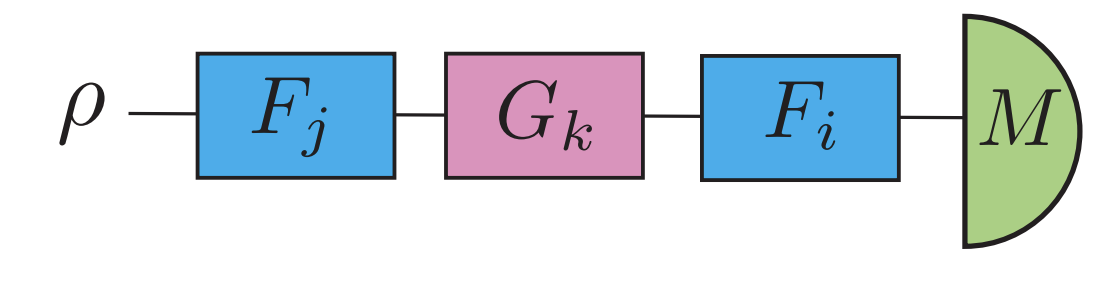
\includegraphics[width=0.35\textwidth]{fig2.png}
\caption{GST circuit: fiducials $F_i$, $F_j$, native gate $G_k$, measurement $M$ on initial state $\rho$.}
\end{figure}

\textcolor{mathpurple}{\textbf{Process matrix parameterization}}: $\chi_G$ has $(D^4 - D^2)/2$ real free params (via Cholesky $\chi_G = T^\dagger T$ + trace-preservation: $\sum_{ij}\chi_{ij}\mathrm{Tr}(E_i E_k E_j) = \delta_{k0}$, giving $D^2$ constraints).

\textbf{Example gate set}: $\{G\} = \{I, \sqrt{X}, \sqrt{Y}\}$, fiducials $\{F\} = \{I, \sqrt{X}, \sqrt{Y}, \sqrt{X}\circ\sqrt{X}\}$. Uses $\sqrt{X}\circ\sqrt{X} = X$ instead of $X$ to reduce cost.

\textbf{Long-sequence GST}: Apply $F_i\, G_k^l\, F_j$ (repeated $l$ times) to \emph{amplify} coherent errors.

\textbf{Resource cost}: 80 experiments for 1 qubit; $>4000$ for 2 qubits; each averaged $\sim 2000$ times.

\begin{minipage}[t]{0.48\textwidth}
\begin{prosbox}
\begin{itemize}
  \item \textcolor{progreen}{\textbf{SPAM-robust}} (models SPAM explicitly)
  \item Full gate set characterization (comprehensive as QPT)
  \item Amplifies coherent errors (long-sequence variant)
  \item Self-consistent: no prior calibration needed
\end{itemize}
\end{prosbox}
\end{minipage}
\hfill
\begin{minipage}[t]{0.48\textwidth}
\begin{consbox}
\begin{itemize}
  \item \textbf{Extremely resource-intensive}: 80+ experiments (1Q), 4000+ (2Q)
  \item Cannot capture non-Markovian noise
  \item Over-complete: much of the data is redundant
  \item Complex classical post-processing (MLE optimization)
\end{itemize}
\end{consbox}
\end{minipage}

\begin{insightbox}
\begin{itemize}
  \item GST is the ``full picture with SPAM included'' --- it's the most complete method but also the most expensive
  \item The gauge freedom is subtle: physically measurable quantities must be gauge-invariant, but the \emph{representation} of the gate set depends on the gauge choice
  \item Key conceptual point: \textbf{fiducial gates serve as an internal reference frame}, eliminating the need for pre-calibrated states or measurements
  \item Recent work has reduced 2-qubit experiments by $\sim 8\times$, but still impractical for many-qubit systems
\end{itemize}
\end{insightbox}

\newpage

% ---------------------------------------------------------------------------
% 3.4 DIRECT FIDELITY ESTIMATION
% ---------------------------------------------------------------------------
\subsection{Direct Fidelity Estimation (DFE)}

\begin{algorithmbox}{DFE Protocol (for gate benchmarking)}
\begin{enumerate}
  \item Define ideal gate $U$ and noisy implementation $\tilde{U}$; their Choi states are $\rho_U$ and $\rho_{\tilde{U}}$
  \item \textbf{Average output fidelity}: $\bar{F}(U, \tilde{U}) = \frac{D\,F_{\mathrm{proc}}(\rho_U, \rho_{\tilde{U}}) + 1}{D + 1}$
  \item Compute directly (no entangled state $|\phi\rangle$ needed):
  \[
    F_{\mathrm{proc}}(\rho_U, \rho_{\tilde{U}}) = \frac{1}{D^4}\sum_{j,k} \mathrm{Tr}(U(P_j)P_k)\;\mathrm{Tr}(\tilde{U}(P_j)P_k)
  \]
  \item Determine tuples $(P_j, P_k)$ for which $\mathrm{Tr}(U(P_j)P_k) \neq 0$; call this set $\mathcal{A}$
  \item \textbf{Importance sampling}: sample from $\mathcal{A}$ with probability $\mathcal{P}(P_j, P_k) = \mathrm{Tr}(U(P_j)P_k)^2/D^4$
  \item For each sample: prepare $D$ eigenstates of $P_j$, apply $\tilde{U}$, measure $P_k$
  \item Average $N$ samples $\Rightarrow$ fidelity estimate $\bar{F}$
\end{enumerate}
\end{algorithmbox}

\begin{figure}[H]
\centering
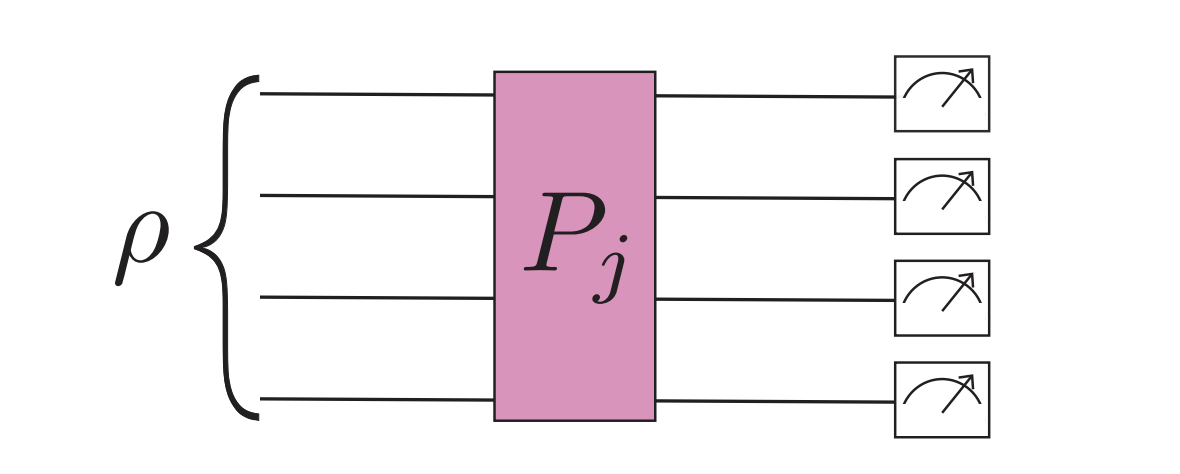
\includegraphics[width=0.3\textwidth]{fig3.png}
\caption{DFE: Estimate state fidelity by sampling random Pauli expectations.}
\end{figure}

\textcolor{mathpurple}{\textbf{Underlying Monte Carlo}}: Fidelity $F(\sigma,\rho) = \mathrm{Tr}(\sigma\rho) = \sum_k p_k x_k = \langle X \rangle$ where $x_k = \rho_k/\sigma_k$, $p_k = \sigma_k^2/D$.

\textbf{Sample complexity}: Worst case exponential in $n$; polynomial for most states of interest. Demonstrated on 7 qubits.

\begin{minipage}[t]{0.48\textwidth}
\begin{prosbox}
\begin{itemize}
  \item No assumptions on noise model
  \item Efficient for most practical states
  \item Only needs local preparations + measurements
  \item No entangled state preparation required
\end{itemize}
\end{prosbox}
\end{minipage}
\hfill
\begin{minipage}[t]{0.48\textwidth}
\begin{consbox}
\begin{itemize}
  \item \textcolor{conred}{\textbf{Susceptible to SPAM errors}}
  \item Worst-case exponential sample complexity
  \item Provides only a single fidelity number
  \item Limited adaptation for routine benchmarking
\end{itemize}
\end{consbox}
\end{minipage}

\newpage

% ---------------------------------------------------------------------------
% 3.5 PROCESS FIDELITY ESTIMATION
% ---------------------------------------------------------------------------
\subsection{Process Fidelity Estimation (PFE)}

\begin{algorithmbox}{PFE Protocol}
\begin{enumerate}
  \item Consider ideal unitary $U$ with projective measurement $\Pi$: ideal map $\Phi = \Pi \circ U$, noisy $\tilde{\Phi} = \Pi \circ \tilde{U}$
  \item Define noise map $\Lambda_U = \tilde{U} \circ U^\dagger$, so $\tilde{U} = \Lambda_U \circ U$
  \item \textcolor{alertred}{\textbf{Key result}}:
  \[
    \boxed{F_{\mathrm{proc}}(\Phi, \tilde{\Phi}) = \frac{1}{D}\sum_{k=1}^{D} \sqrt{\Pr\!\left(k \,|\, \Lambda_U(\pi_k)\right)} = \frac{1}{D}\sum_{k=1}^{D} \sqrt{\langle k|\tilde{U}(U^\dagger(\pi_k))|k\rangle}}
  \]
  \item \textbf{Operational meaning}: Prepare time-reversed states $|\psi_k\rangle = U^\dagger|k\rangle$, then apply $\tilde{U}$, measure prob.\ of outcome $k$
  \item \textbf{Unbiased estimator} (via sampling $m$ values of $k$):
  \[
    F_{\mathrm{proc}} \approx \frac{m}{m-1}\left(\frac{1}{m}\sum_{l=1}^m \sqrt{\Pr(k_l|\Lambda_U(\pi_{k_l}))}\right)^2 - \frac{1}{m(m-1)}\sum_{l=1}^m \Pr(k_l|\Lambda_U(\pi_{k_l}))
  \]
\end{enumerate}
\end{algorithmbox}

\begin{minipage}[t]{0.48\textwidth}
\begin{prosbox}
\begin{itemize}
  \item Generalizes DFE to include measurements (applicable to entire algorithms)
  \item No entangled state preparation needed
  \item Unitarily invariant fidelity
\end{itemize}
\end{prosbox}
\end{minipage}
\hfill
\begin{minipage}[t]{0.48\textwidth}
\begin{consbox}
\begin{itemize}
  \item Requires preparing time-reversed states $U^\dagger|k\rangle$ with high fidelity
  \item Exponentially many initial states (must sample)
  \item $O(1/m)$ bias in naive estimator
\end{itemize}
\end{consbox}
\end{minipage}

\begin{insightbox}
\begin{itemize}
  \item PFE's conceptual innovation: by including the measurement in the benchmark, it captures \emph{end-to-end} circuit performance
  \item The key equation derives from Choi state analysis + the fact that $\rho_\Pi^2 = \rho_\Pi / D$ (projectors on computational basis are pure)
  \item The time-reversed state preparation $U^\dagger|k\rangle$ can sometimes be done with only Hadamard + virtual phase gates
\end{itemize}
\end{insightbox}

\newpage

% ---------------------------------------------------------------------------
% 3.6 CROSS-ENTROPY BENCHMARKING
% ---------------------------------------------------------------------------
\subsection{Cross-Entropy Benchmarking (XEB)}

\begin{algorithmbox}{XEB / RCS Benchmarking Protocol}
\begin{enumerate}
  \item \textbf{Sample} random circuit $C_i$ from ensemble $\mathrm{RCS}(n, P)$: $P$ layers of 2-qubit gates interleaved with Haar-random 1-qubit gates
  \item \textbf{Run} noisy circuit $\tilde{C}_i$ on quantum hardware; collect $M$ bitstring samples $\{x_i\}_{i=1}^M$
  \item \textbf{Classically simulate} ideal circuit to get $p_U(x_i)$ for each sampled bitstring
  \item \textbf{Estimate fidelity} via \textcolor{alertred}{linear cross-entropy}:
  \[
    \boxed{\hat{F}_{\mathrm{XEB}} = \frac{D}{M}\sum_{i=1}^M p_U(x_i) - 1}
  \]
  \item \textbf{Repeat} for $L$ random circuits; average: $\hat{F}_P = \frac{1}{L}\sum_i \hat{F}_{P,i}$
  \item \textbf{Repeat} for varying depths $P \in \{1,\ldots,P_{\max}\}$
  \item \textbf{Fit}: $\hat{F}_P = A\,e^{-\lambda P}$, extract noise strength $\lambda = \sum_\alpha p_\alpha$ (Pauli error rates)
\end{enumerate}
\end{algorithmbox}

\begin{figure}[H]
\centering
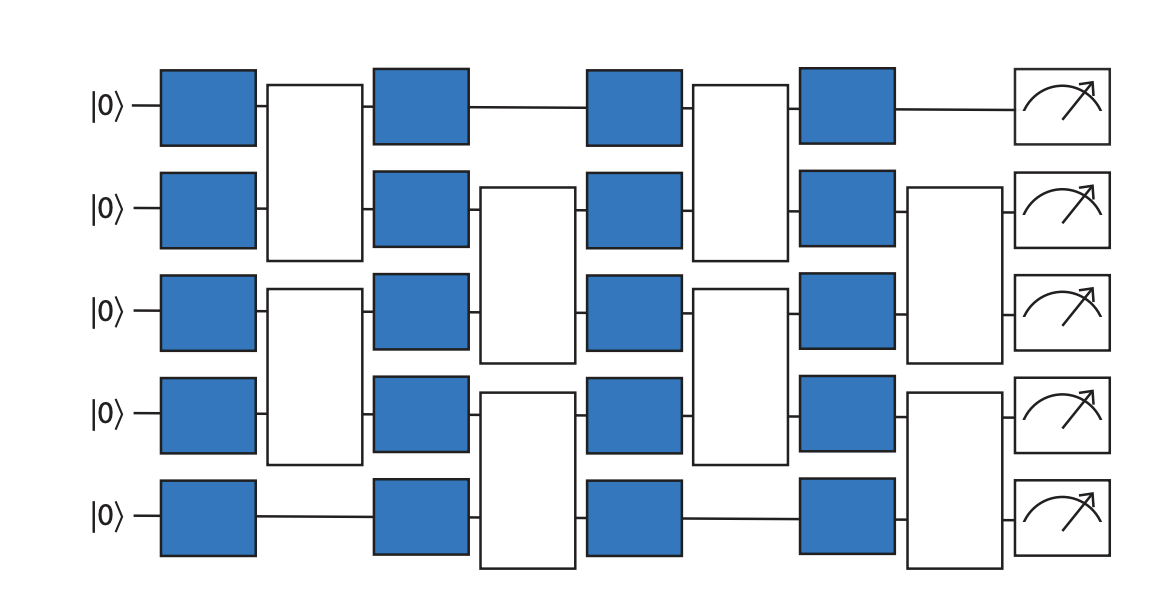
\includegraphics[width=0.5\textwidth]{fig4.png}
\caption{RCS benchmarking circuit: layers of 2-qubit gates (white) interleaved with Haar-random 1-qubit gates (blue), followed by measurement.}
\end{figure}

\textcolor{mathpurple}{\textbf{Noise model}}: $\rho_{\tilde{U}} = F_U |\psi_U\rangle\langle\psi_U| + (1-F_U)\sigma_U$. \textbf{Central assumption}: for deep random circuits, $\mathbb{E}_U[p_{\sigma_U}] \approx$ uniform distribution (concentration of measure).

\textbf{Unbiased estimator}: $\hat{F}_{\mathrm{uXEB}} = \frac{(D/M)\sum_i p_U(x_i) - 1}{D\sum_x p_U(x)^2 - 1}$ (denominator $\to 1$ at $\log$ depth for random circuits).

\textbf{Variance}: $\mathrm{Var}(\hat{F}_{\mathrm{uXEB}}) = O(1/M) + \lambda^2(\mathbb{E}[F])^2$ $\Rightarrow$ needs $M = O(1/\epsilon^2)$ samples per circuit.

\begin{minipage}[t]{0.48\textwidth}
\begin{prosbox}
\begin{itemize}
  \item Scales to $\sim$50 qubits (limited by classical simulation)
  \item SPAM-robust (depth-independent fit params)
  \item \textbf{Sample-efficient}: $O(1/\epsilon^2)$ measurements per circuit
  \item Works with arbitrary non-Clifford gates
  \item Basis for quantum supremacy experiments
\end{itemize}
\end{prosbox}
\end{minipage}
\hfill
\begin{minipage}[t]{0.48\textwidth}
\begin{consbox}
\begin{itemize}
  \item Requires \textbf{classical simulation} of ideal circuit (infeasible for very large circuits)
  \item Insensitive to $I/Z$ errors (don't affect computational basis measurements)
  \item Not a good fidelity proxy for time-correlated errors
  \item Strong assumption: noise depends on gates but not their order
  \item Single aggregate error metric (no specificity)
\end{itemize}
\end{consbox}
\end{minipage}

\begin{insightbox}
\begin{itemize}
  \item XEB was designed for the quantum supremacy regime: the \emph{idea} is that if a noisy circuit produces bitstrings whose ideal probabilities are higher than chance, it's computing something
  \item \textbf{Porter--Thomas distribution}: for random circuits, the ideal output probabilities follow an exponential distribution --- this is essential for XEB to work, as it provides the variance structure needed
  \item XEB's blindness to $I/Z$ errors is a significant limitation: in the computational basis, a $Z$ error changes only the phase and not the measurement outcome
  \item RCS benchmarking mirrors RB's structure: random circuits play the role of random Cliffords, and the exponential decay is analogous
\end{itemize}
\end{insightbox}

\newpage

% ===========================================================================
% SECTION 4: DETERMINISTIC BENCHMARKING
% ===========================================================================
\section{Deterministic Benchmarking (DB) -- Novel Contribution}

\begin{figure}[H]
\centering
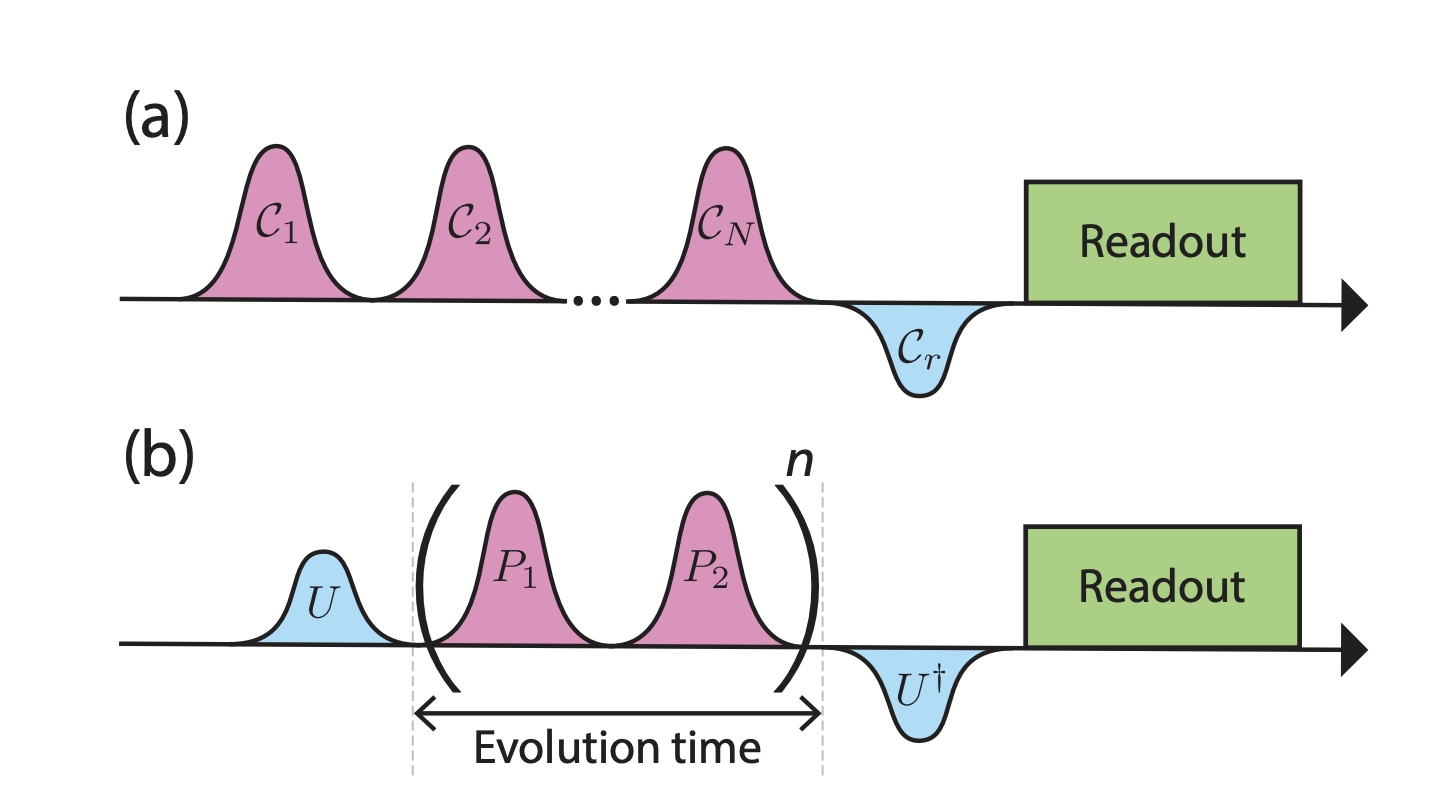
\includegraphics[width=0.7\textwidth]{fig5.png}
\caption{RB vs.\ DB: (a) RB uses $N$ random Cliffords $\mathcal{C}_i$ + recovery $\mathcal{C}_r$; (b) DB uses state prep $U$, $n$ repetitions of fixed pulse-pair $P_1 P_2$, un-prep $U^\dagger$.}
\end{figure}

\subsection{Qubit Model}

\begin{itemize}
  \item Transmon qubit modeled as \textbf{driven two-level system} in the drive frame (rotating wave approximation)
  \item Hamiltonian generating gates $R_x(\theta)$, $R_y(\theta)$:
  \begin{equation}
    H_\alpha = (\varepsilon + \varepsilon_{\mathrm{err}})\frac{\sigma_\alpha}{2} + \Delta_{\mathrm{err}}\frac{\sigma_z}{2}, \qquad \alpha \in \{x, y\}
  \end{equation}
  \item \textbf{Rotation error}: $\delta\theta \equiv \varepsilon_{\mathrm{err}}\, t_g$ \quad (amplitude error $\times$ gate time)
  \item \textbf{Phase error}: $\delta\phi \equiv \Delta_{\mathrm{err}}/\bar{\varepsilon} = \Delta_{\mathrm{err}}\, t_g / \theta$ \quad (detuning relative to drive)
  \item $\Delta_{\mathrm{err}}$ arises from both detuning and ac-Stark shift from driving higher transitions
\end{itemize}

\subsection{Four Key Parameters}

While a general single-qubit CPTP map has 12 parameters, DB reduces to \textcolor{alertred}{\textbf{4 key parameters}}: $\{T_1, T_2, \delta\theta, \delta\phi\}$

\begin{keybox}
\begin{center}
\begin{tabular}{llll}
\toprule
\textbf{Parameter} & \textbf{Type} & \textbf{Physical Origin} & \textbf{DB Sequence} \\
\midrule
$T_1$ & Incoherent & Relaxation to equilibrium & Free evolution; $|1\rangle$ \\
$T_2$ & Incoherent & Coherence time ($1/T_2 = 1/2T_1 + 1/T_\phi$) & $XX$; $|+\rangle$ \\
$\delta\theta$ & Coherent & Rotation (amplitude) error & $YY$; $|+\rangle$ \\
$\delta\phi$ & Coherent & Phase (detuning) error & $X\bar{X}$; $|+\rangle$ \\
\bottomrule
\end{tabular}
\end{center}
\end{keybox}

\textbf{Gate-pair sequences}: $P_1 P_2 \in \{XX, X\bar{X}, YY, Y\bar{Y}, \bar{Y}Y\}$, where $X \equiv R_x(\pi)$, $\bar{X} \equiv R_x(-\pi)$, etc. Without errors: $P_1 P_2 = \pm I$.

\subsection{DB Protocol}

\begin{algorithmbox}{Deterministic Benchmarking Protocol}
\textbf{Universal fidelity expression}: In all experiments, the fidelity is accurately described by:
\[
  \boxed{F(t_n) = \frac{1}{2}(1+a) + \frac{1}{2}(1-a)\,e^{-t_n/T_D}\cos(2\omega t_n)}
\]
where $t_n = 2n\,t_g$, $T_D$ = decay timescale (incoherent), $\omega$ = oscillation frequency (coherent), $a$ = deviation from infinite-$T$ limit.

\textbf{Learning experiments} (Steps 1--4):
\begin{enumerate}
  \item $\{\mathrm{free};\; |1\rangle\}$: Standard $T_1$ measurement. $F = \frac{1}{2}(1+a) + \frac{1}{2}(1-a)e^{-t/T_1}$ $\Rightarrow$ extract $\textcolor{alertred}{T_1}$
  \item $\{XX;\; |+\rangle\}$: Exponential decay $\Rightarrow$ extract $\textcolor{alertred}{T_2}$ (analogous to echo-Ramsey). $T_\phi = 2T_1 T_2/(2T_1 - T_2)$
  \item $\{YY;\; |+\rangle\}$: Oscillations $\Rightarrow$ fit to find $\textcolor{alertred}{\delta\theta}$ where $\omega \approx \delta\theta/(2t_g)$
  \item $\{X\bar{X};\; |+\rangle\}$: Oscillations $\Rightarrow$ fit to find $\textcolor{alertred}{\delta\phi}$ where $\omega = \delta\phi/t_g$
\end{enumerate}

\textbf{Test experiments} (Steps 5--6):
\begin{enumerate}[resume]
  \item $\{Y\bar{Y};\; |+\rangle\}$ and $\{\bar{Y}Y;\; |+\rangle\}$: Tests interplay of relaxation and gate operations; validates $\{T_1,T_2,\delta\theta,\delta\phi\}$; can characterize qubit temperature
  \item Various (e.g., UR6 DD sequence): Further validation; UR6 suppresses coherent errors
\end{enumerate}

\textbf{Notation}: $\{P_1 P_2;\; |\psi\rangle\}$ means: prepare $|\psi\rangle$ from $|0\rangle$, apply $(P_1 P_2)^n$, un-prepare $|\psi\rangle$, measure in $\sigma_z$ basis.
\end{algorithmbox}

\subsection{Experimental Results}

\textbf{Device}: Superconducting grounded Xmon transmon, dispersively coupled to CPW readout resonator. DRAG-calibrated pulses, cosine envelope, $t_g = 88$ ns (80 ns pulse + 8 ns padding).

\begin{keybox}
\centering\small
\begin{tabular}{cccccc}
\toprule
$\omega_q/2\pi$ & $|\eta|/2\pi$ & $\chi_{qc}/2\pi$ & $\omega_c/2\pi$ & $T_1$ & $T_2^*$ \\
\midrule
4.37 GHz & 215 MHz & 230 kHz & 6.95 GHz & 20 $\mu$s & 32 $\mu$s \\
\bottomrule
\end{tabular}
\end{keybox}
\vspace{2pt}

\begin{figure}[H]
\centering
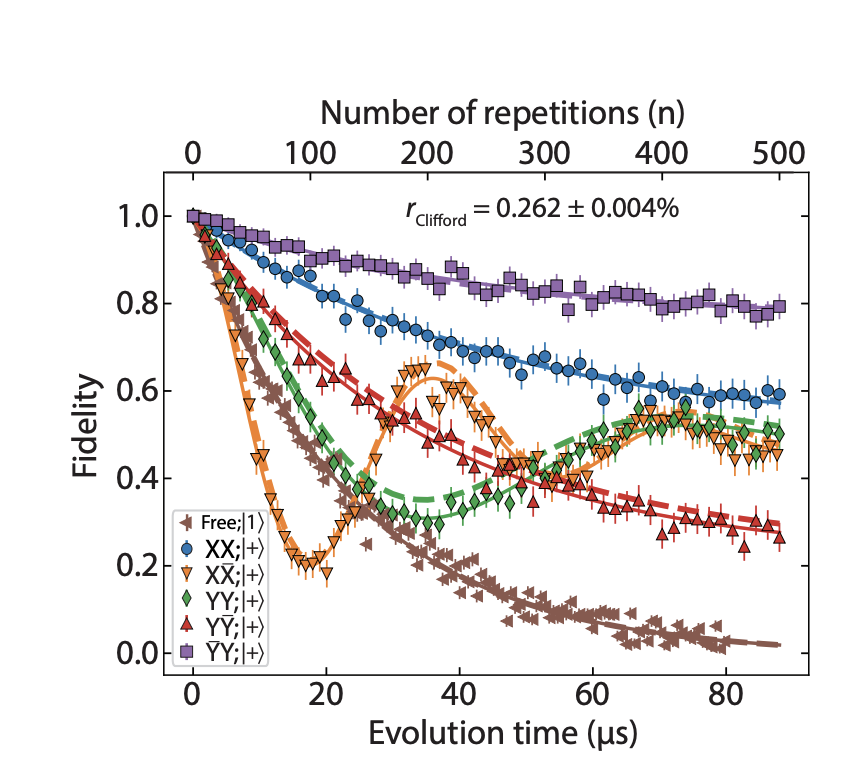
\includegraphics[width=0.55\textwidth]{fig6.png}
\caption{DB fidelities: symbols = experiment, solid = analytical fit [Eq.~above], dashed = Lindblad simulation. Extracted: $T_1 = 23.36\pm0.40\;\mu$s, $T_2 = 44.13\pm2.49\;\mu$s, $\delta\theta = 0.398\pm0.004^\circ$, $\delta\phi = 0.426\pm0.004^\circ$.}
\end{figure}

\begin{figure}[H]
\centering
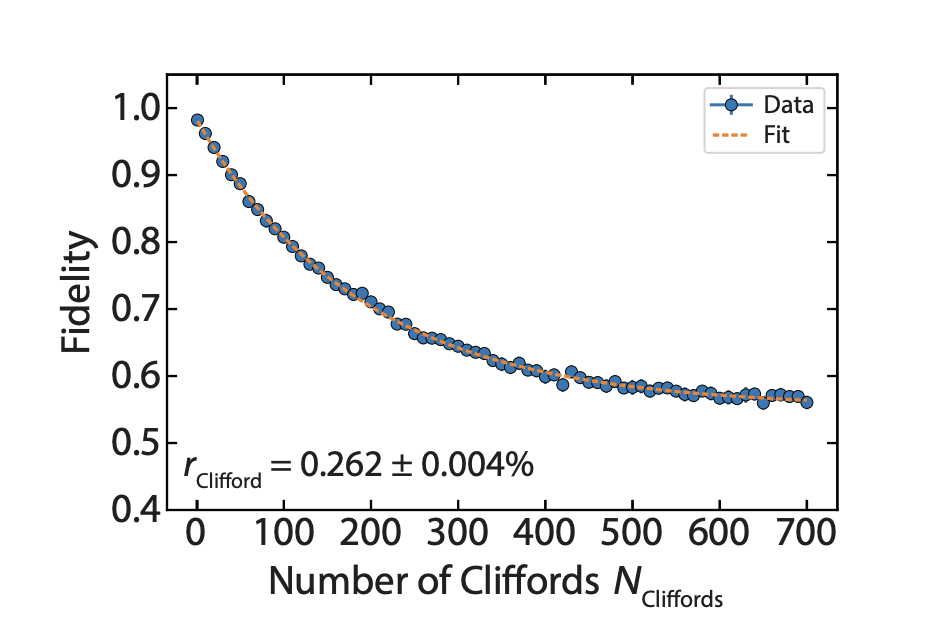
\includegraphics[width=0.4\textwidth]{fig7.png}
\caption{RB for same parameters: $r_C = 0.262\pm0.004\%$ over 30 random sequences with up to 700 Cliffords. RB misses the coherent oscillations and $T_1$/$T_2$ distinction.}
\end{figure}

\textcolor{alertred}{\textbf{Key observations:}}
\begin{itemize}
  \item $YY$ oscillates $\Rightarrow$ rotation errors; $X\bar{X}$ oscillates $\Rightarrow$ phase errors
  \item $XX$ on $|+\rangle$ is insensitive to coherent errors: pure exponential decay $\Rightarrow$ $T_2$
  \item Strong \textbf{asymmetry} between $Y\bar{Y}$ and $\bar{Y}Y$: $Y\bar{Y}$ confines state to southern (excited) hemisphere $\Rightarrow$ faster decay; $\bar{Y}Y$ stays in northern hemisphere
  \item RB gives $r_C = 0.262\%$ --- a single number that misses all this structure
\end{itemize}

\subsection{Closed-System (Coherent Error) Fidelities}

\textcolor{mathpurple}{\textbf{Analytical results}} for initial state $|+\rangle$, $\theta_{\mathrm{err}} \equiv \sqrt{(\varepsilon t_g + \delta\theta)^2 + (\pi\delta\phi)^2}$:
\begin{align}
  F_{YY}^{\mathrm{clsd}}(n) &= \cos^2(n\,\theta_{\mathrm{err}}) \xrightarrow{\text{small errors}} \cos^2(n\,\delta\theta) & \text{\textcolor{alertred}{dominated by $\delta\theta$}} \\
  F_{XX}^{\mathrm{clsd}}(n) &= 1 - \left(\frac{\pi\delta\phi\sin(n\theta_{\mathrm{err}})}{\theta_{\mathrm{err}}}\right)^2 \xrightarrow{\text{small errors}} 1 & \text{insensitive to errors} \\
  F_{X\bar{X}}^{\mathrm{clsd}}(n) &= \cos^2(n\,\phi_{\mathrm{err}}) \xrightarrow{\text{small errors}} \cos^2\!\left(\tfrac{1}{2}n\delta\phi[1 - \pi\delta\theta]\right) & \text{\textcolor{alertred}{dominated by $\delta\phi$}}
\end{align}

\subsection{Open System Model}

\textbf{Lindblad master equation}: $\partial_t \rho = \mathcal{L}(\rho) = -i[H,\rho] + \sum_\alpha \frac{\gamma_\alpha}{2}(L_\alpha \rho L_\alpha^\dagger - \{L_\alpha^\dagger L_\alpha, \rho\})$

Lindblad operators: $L_1 = \sigma^- = |0\rangle\langle 1|$ ($\gamma_1 = 1/T_1$), $L_\phi = \sigma_z/\sqrt{2}$ ($\gamma_\phi = 1/T_\phi$).

Using fitted $\{T_1, T_2, \delta\theta, \delta\phi\}$ from Steps 1--4 $\Rightarrow$ Lindblad simulations predict Steps 5--6 \textcolor{alertred}{accurately} (dashed curves in Fig.~6).

\subsection{Sensitivity to Coherent Errors}

\begin{figure}[H]
\centering
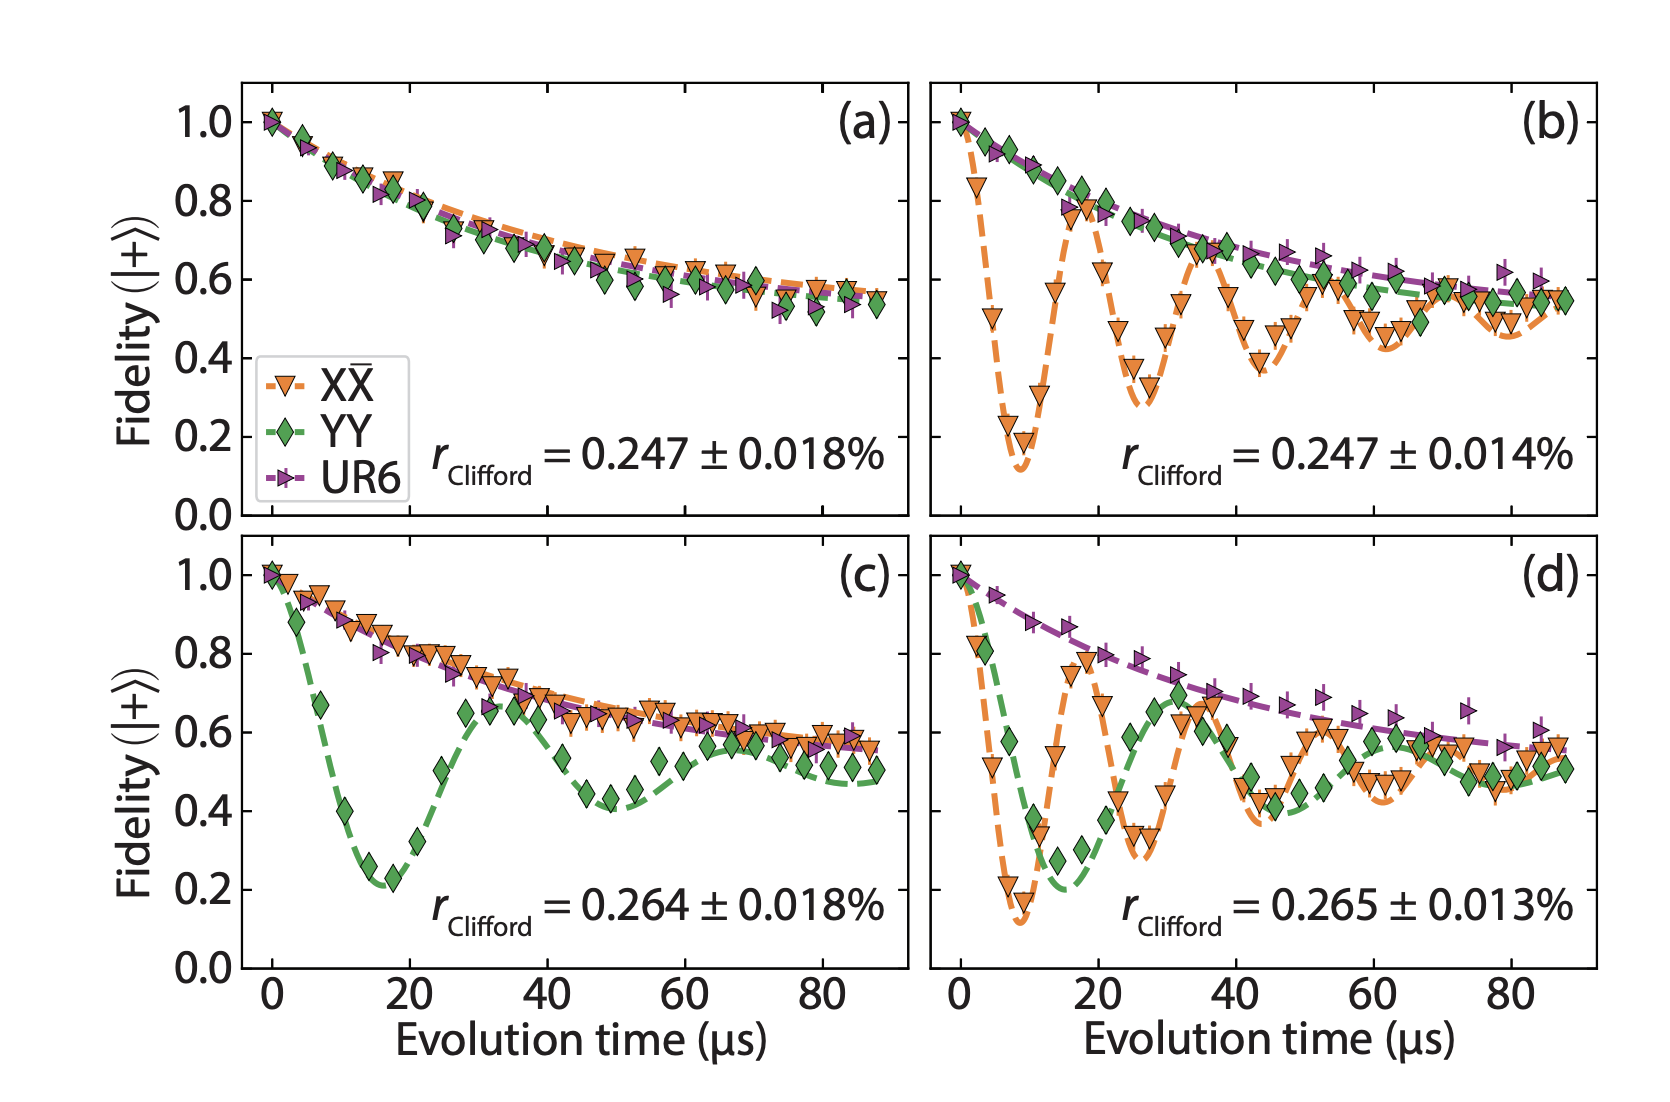
\includegraphics[width=0.65\textwidth]{fig8.png}
\caption{Sensitivity comparison DB vs.\ RB: (a) calibrated gates ($\delta\theta = \delta\phi = 0$), (b) phase error only, (c) rotation error only, (d) both errors. \textcolor{alertred}{RB's $r_C$ is essentially unchanged} despite significant coherent errors visible in DB.}
\end{figure}

\textcolor{alertred}{\textbf{Critical finding}}: Small coherent errors ($\delta\phi \approx 0.9^\circ$, $\delta\theta \approx 0.93^\circ$) cause large, rapid oscillations in DB fidelity, while \textbf{RB's $r_C$ changes by $< 0.02\%$}. This demonstrates RB's fundamental limitation.

\textbf{UR6 sequence} never exhibits oscillations $\Rightarrow$ confirms oscillations are from coherent errors (UR6 suppresses them by design).

\textbf{Induced rotation error} from detuning: $\delta\theta_{\mathrm{ind}} \approx \frac{1}{2}\varphi\,\delta\phi^2$ (negligible for small $\delta\phi$).

\subsection{\texorpdfstring{$T_1$}{T1} Asymmetry and Temperature}

\begin{figure}[H]
\centering
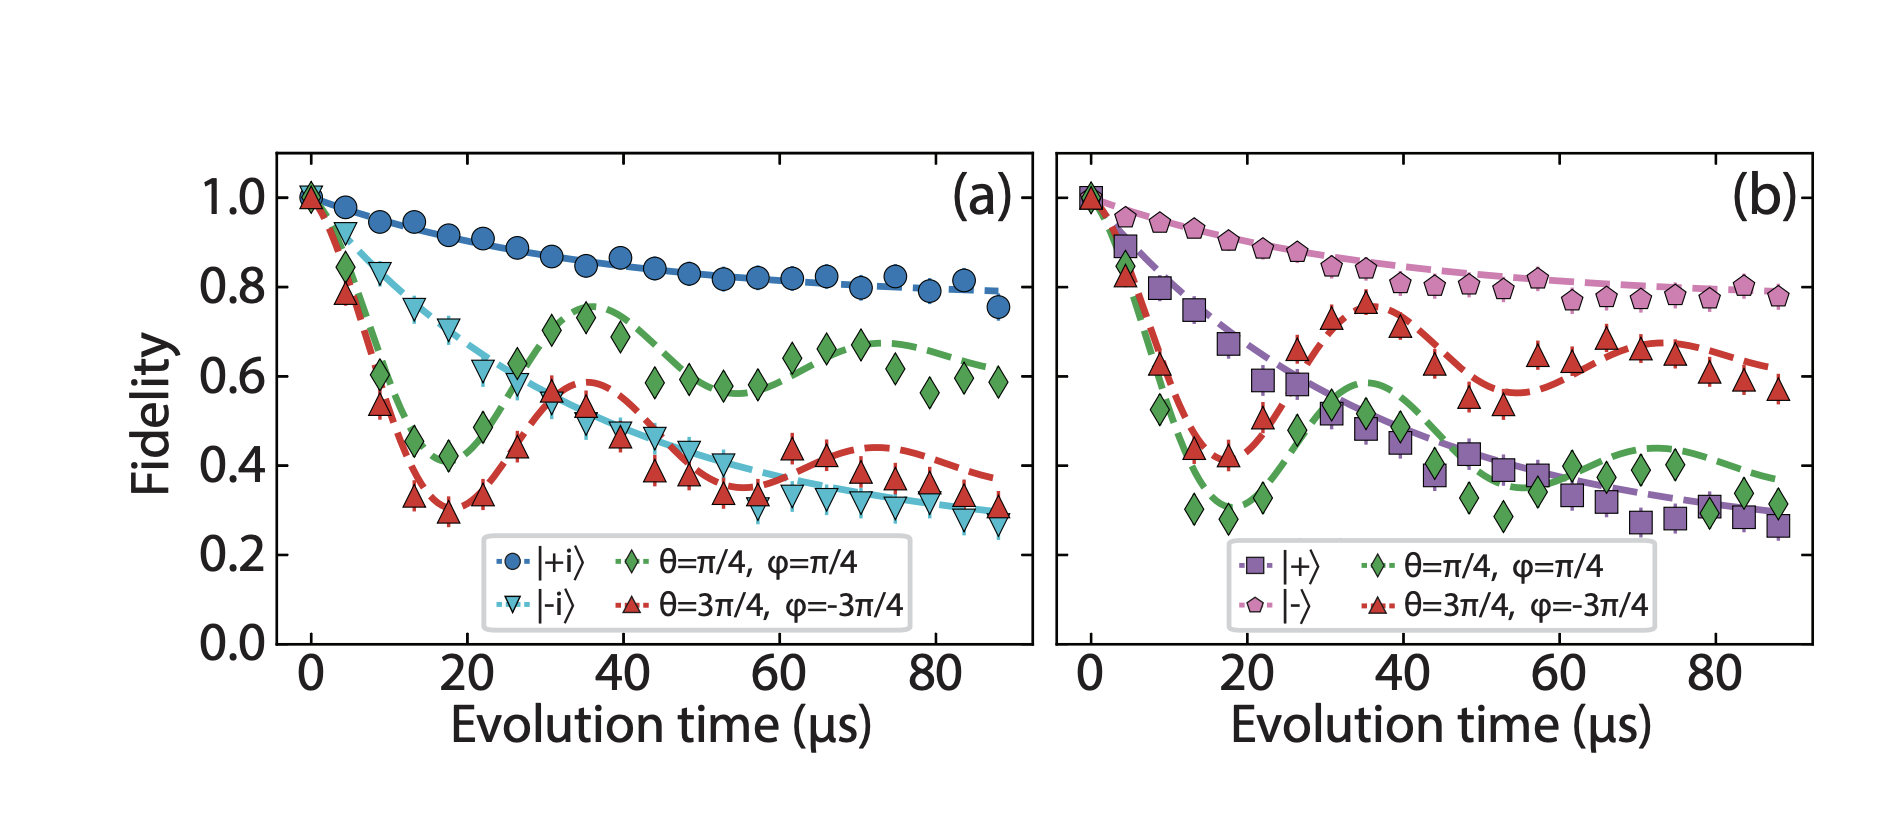
\includegraphics[width=0.6\textwidth]{fig9.png}
\caption{Asymmetric decay under (a) $XX$ on $|\pm i\rangle$ and other states, (b) $YY$ on $|\pm\rangle$ and other states. Orthogonal states show opposite asymmetry due to hemisphere confinement.}
\end{figure}

\begin{itemize}
  \item Transmon operates at $\omega_{01} \in [3{-}6]$ GHz, $T \sim 10$ mK ($\sim 0.2$ GHz) $\Rightarrow$ ground state $\approx$ thermal state
  \item $Y\bar{Y}$ confines state to \textbf{southern hemisphere} (excited) $\Rightarrow$ susceptible to $T_1$ relaxation $\Rightarrow$ faster decay
  \item $\bar{Y}Y$ confines to \textbf{northern hemisphere} (ground) $\Rightarrow$ less relaxation $\Rightarrow$ slower decay, higher saturation
  \item This asymmetry enables \textbf{temperature calibration}: $k_BT = \omega_{01}\left[\ln\!\left(\frac{a_{T=0} + a}{a_{T=0} - a}\right)\right]^{-1}$
  \item Choose pulse sequences with larger $|a_{T=0}|$ (e.g., $Y\bar{Y}$) for more sensitive temperature measurement
\end{itemize}

\subsection{Analytical Derivations}

\subsubsection{Bloch Vector Formulation}

$\rho = \frac{1}{2}(I + v_x\sigma_x + v_y\sigma_y + v_z\sigma_z)$, \; $H = \frac{1}{2}(h_x\sigma_x + h_y\sigma_y + h_z\sigma_z)$

Dissipator: $R = \mathrm{diag}(-\gamma_2, -\gamma_2, -\gamma_1)$, $c = (0,0,\eta\gamma_1)$, with $\gamma_2 = \frac{1}{2}\gamma_1 + \gamma_\phi$ and $\eta = \frac{1 - e^{-\beta\omega_{01}}}{1 + e^{-\beta\omega_{01}}} \in [0,1]$.

\textbf{Bloch equation}: $\dot{v} = h \times v + Rv + c$. \quad Fidelity with $|+\rangle$: $F(t) = \frac{1}{2}(1 + v_x(t))$.

\subsubsection{\texorpdfstring{YY Sequence ($\Delta_{\mathrm{err}} = 0$)}{YY Sequence (Delta\_err = 0)}}

For square $YY$ pulse, $h = (0, \varepsilon_{\mathrm{tot}}, 0)$. Solving $\dot{v} = Gv + c$ with $v(0) = (1,0,0)$:
\begin{align}
  v_\infty &= \eta\frac{\varepsilon_{\mathrm{tot}}^2\gamma_1}{\varepsilon_{\mathrm{tot}}^2 + \gamma_1\gamma_2}, \quad \gamma_* = \frac{1}{2}(\gamma_1 + \gamma_2), \quad \omega_* = \sqrt{\varepsilon_{\mathrm{tot}}^2 - \frac{1}{4}(\gamma_1 - \gamma_2)^2}
\end{align}

In the regime $\varepsilon \gg \varepsilon_{\mathrm{err}}, \gamma_1, \gamma_2$: $v_\infty \approx \eta\gamma_1/\varepsilon$, $\omega_* \approx \varepsilon_{\mathrm{tot}}$:
\begin{equation}
  \textcolor{alertred}{F_{\delta\phi=0}(t_n) = \frac{1}{2}(1+v_\infty) + \frac{1}{2}(1-v_\infty)e^{-\gamma_* t_n}\cos(2n\delta\theta)}
\end{equation}
This matches the phenomenological form exactly: $a = v_\infty$, $T_D = 1/\gamma_*$, $2\omega t_g = \delta\theta$.

For $\Delta_{\mathrm{err}} \neq 0$: perturbative correction $|F_{YY}(n) - F_{\delta\phi=0}(n)| = O(\gamma_1/\varepsilon) = O(\gamma_1 t_g)$.

\subsubsection{XX Sequence}

For the simplified model $\gamma_1 = \gamma_2 = \gamma$ (i.e., $T_\phi = 2T_1$), the Bloch vector after $n$ XX pulse-pairs satisfies a recurrence $v(2(n+1)t_g) = Av(2nt_g) - \zeta$. Under first-order approximations:
\begin{equation}
  \textcolor{alertred}{F(t_n) = \frac{1}{2} + \frac{1}{2}e^{-\gamma t_n}\cos(2n\vartheta)}, \quad \vartheta = \tan^{-1}\!\left(2\sin\frac{\omega' t_g}{2}\cdot\frac{\Delta_{\mathrm{err}}}{\omega'}\right)
\end{equation}
where $\omega' = \sqrt{\varepsilon_{\mathrm{tot}}^2 + \Delta_{\mathrm{err}}^2}$, and the oscillation frequency matches the closed-system result.

\subsection{Leakage Diagnostics}

\begin{figure}[H]
\centering
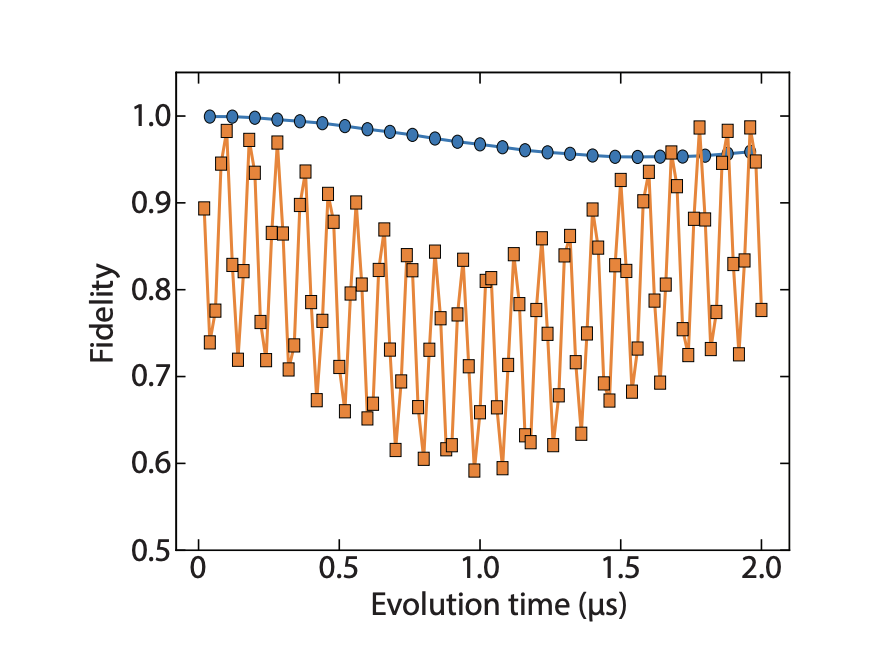
\includegraphics[width=0.4\textwidth]{fig10.png}
\caption{Simulated fidelity of $|+\rangle$ under $XX$ with leakage to a state $-150$ MHz detuned. 20 ns pulses (blue) show minimal leakage; 10 ns pulses (orange) show significant oscillations. DRAG can remove these.}
\end{figure}

\begin{itemize}
  \item $XX$ on $|+\rangle$ has \emph{no oscillations} absent leakage $\Rightarrow$ any oscillations in $XX$ are a \textbf{direct leakage diagnostic}
  \item Faster gates (larger bandwidth) $\Rightarrow$ more leakage $\Rightarrow$ larger/faster oscillations
  \item DRAG pulse optimization can suppress leakage; residual leakage detectable via DB
  \item Useful when leakage state is unknown (direct population measurement impossible)
\end{itemize}

\subsection{DB Summary}

\begin{minipage}[t]{0.48\textwidth}
\begin{prosbox}
\begin{itemize}
  \item \textbf{Only 4 experiments} needed (vs.\ 80+ for GST, $D^4$ for QPT)
  \item \textbf{SPAM-resilient} (exponential decay separates SPAM)
  \item Detects \textbf{coherent errors invisible to RB}
  \item Distinguishes $T_1$ from $T_2$
  \item Enables \textbf{temperature calibration}
  \item Enables \textbf{leakage diagnostics}
  \item Simple analytical model; Lindblad validation
  \item Platform-independent (validated on transmon)
\end{itemize}
\end{prosbox}
\end{minipage}
\hfill
\begin{minipage}[t]{0.48\textwidth}
\begin{consbox}
\begin{itemize}
  \item \textbf{Currently limited to single-qubit gates}
  \item 4 parameters (not full 12-parameter CPTP characterization)
  \item Assumes Markovian noise model
  \item Extension to 2-qubit gates is an open problem
  \item Not yet widely adopted/tested
\end{itemize}
\end{consbox}
\end{minipage}

\begin{insightbox}
\begin{itemize}
  \item DB's philosophy: \emph{target the right physics} rather than brute-force characterize everything
  \item The choice of $XX$, $YY$, $X\bar{X}$ sequences is not arbitrary --- each isolates one specific error type by exploiting the qubit's Bloch sphere geometry
  \item $XX$ on $|+\rangle$: the state remains at $|+\rangle$ under ideal noiseless evolution $\Rightarrow$ any decay is purely incoherent $\Rightarrow$ clean $T_2$ measurement
  \item The $Y\bar{Y}$ vs.\ $\bar{Y}Y$ asymmetry is deeply physical: it reflects the asymmetry between absorption and emission at finite temperature, modulated by where the pulse sequence keeps the state on the Bloch sphere
  \item DB's connection to \textbf{dynamical decoupling}: same pulse sequences, but DD tries to \emph{suppress} noise while DB tries to \emph{characterize} it --- a clever inversion of purpose
  \item The phenomenological fidelity $F(t_n) = \frac{1}{2}(1+a) + \frac{1}{2}(1-a)e^{-t_n/T_D}\cos(2\omega t_n)$ naturally emerges from the Lindblad equation, validating the 4-parameter model
  \item \textbf{Noise bias} revealed by DB (asymmetry in relaxation during gates) could inform compilation strategies that minimize time spent near excited states
\end{itemize}
\end{insightbox}

\newpage

% ===========================================================================
% SECTION 5: CONCLUSIONS & COMPARISON TABLE
% ===========================================================================
\section{Conclusions and Method Comparison}

\begin{table}[H]
\centering
\small
\renewcommand{\arraystretch}{1.15}
\begin{tabularx}{\textwidth}{l|c|c|c|c|c|c|X}
\toprule
\textbf{Method} & \textbf{Params} & \textbf{SPAM} & \textbf{Coherent} & \textbf{Scaling} & \textbf{Cost} & \textbf{Scope} & \textbf{Key Use Case} \\
\midrule
\textcolor{deepblue}{\textbf{RB}} & 1 & \textcolor{progreen}{robust} & \textcolor{conred}{no} & good & low & gate & Quick fidelity check \\
\textcolor{deepblue}{\textbf{IRB}} & 1 & \textcolor{progreen}{robust} & \textcolor{conred}{no} & good & low & gate & Specific gate fidelity \\
\textcolor{deepblue}{\textbf{SQPT}} & $D^4{-}D^2$ & \textcolor{conred}{sensitive} & \textcolor{progreen}{yes} & poor & high & gate & Full characterization \\
\textcolor{deepblue}{\textbf{AAPT}} & $D^4{-}D^2$ & \textcolor{conred}{sensitive} & \textcolor{progreen}{yes} & poor & high & gate & Full char.\ w/ ancilla \\
\textcolor{deepblue}{\textbf{DCQD}} & $D^4{-}D^2$ & \textcolor{keyorange}{partial} & \textcolor{progreen}{yes} & moderate & mod. & gate & Efficient full char. \\
\textcolor{deepblue}{\textbf{GST}} & $D^4{-}D^2$ & \textcolor{progreen}{robust} & \textcolor{progreen}{yes} & poor & v.\ high & gate set & Gold standard + SPAM \\
\textcolor{deepblue}{\textbf{DFE}} & 1 & \textcolor{conred}{sensitive} & \textcolor{progreen}{yes} & moderate & mod. & gate/circ. & Fidelity estimation \\
\textcolor{deepblue}{\textbf{PFE}} & 1 & \textcolor{keyorange}{partial} & \textcolor{progreen}{yes} & moderate & mod. & circuit & End-to-end fidelity \\
\textcolor{deepblue}{\textbf{XEB}} & 1 & \textcolor{progreen}{robust} & \textcolor{conred}{partial} & good & mod. & circuit & Supremacy; noise rate \\
\textcolor{alertred}{\textbf{DB}} & 4 & \textcolor{progreen}{robust} & \textcolor{progreen}{yes} & 1Q only & \textcolor{progreen}{v.\ low} & gate & Coherent + incoherent \\
\bottomrule
\end{tabularx}
\caption{Comparison of benchmarking methods. Color coding: \textcolor{progreen}{green} = advantage, \textcolor{conred}{red} = disadvantage, \textcolor{keyorange}{orange} = partial.}
\end{table}

\textbf{Key takeaways:}
\begin{itemize}
  \item \textbf{No universal winner}: method choice depends on goal (calibration, performance prediction, processor quality)
  \item \textbf{RB} = cheapest but least informative; \textbf{GST/QPT} = most informative but most expensive
  \item \textbf{DB} fills a gap: more informative than RB, much cheaper than GST, detects coherent errors
  \item \textbf{XEB} is unique in scaling to large systems but requires classical simulability
  \item Noise-reduction strategies (error mitigation, QEC) \emph{require} accurate noise characterization $\Rightarrow$ benchmarking is a prerequisite for fault tolerance
  \item Open problem: extending DB to 2-qubit gates with minimal parameter set
\end{itemize}

\begin{insightbox}
\begin{itemize}
  \item \textbf{Expert strategy}: Use RB for quick monitoring, DB for detailed single-qubit calibration, GST when you need the full picture and can afford the cost, XEB for circuit-level assessment
  \item \textbf{Coherent errors are the silent killer}: they accumulate quadratically, are invisible to RB, and can dominate in well-engineered devices where incoherent errors have been minimized
  \item \textbf{Benchmarking $\neq$ characterization}: benchmarking gives metrics, characterization gives the error map. Choose based on whether you need to \emph{compare} or \emph{fix} the gate
  \item As quantum chemistry pushes toward chemical accuracy, the demands on gate fidelity will increase dramatically --- benchmarking methods must evolve correspondingly
\end{itemize}
\end{insightbox}

\end{document}
